\documentclass[10pt,xcolor={table,dvipsnames},t]{beamer}
\usetheme{UCBerkeley}
\usepackage{ctex}
\bibliography{ref}
\newcommand{\his}{\textsuperscript{\ddag}}

\title{Turbulence phenomenology}
\subtitle{The Gioia\his way.}
\author{刘宁}
\institute{浙江大学}
\date{\today}

\begin{document}

\begin{frame}
  \titlepage
\end{frame}

\begin{frame}{Velocity component at $s$ scale}
    \begin{align*}
        u_s^2 = \int_0^s E(\sigma) \sigma^{-2} d\sigma = \int_{1 / s}^{\infty} E(k) dk
    .\end{align*}
    with $E(\sigma) \sim \varepsilon^{2 / 3} \sigma^{5 / 3} \mathbf{c_d} \left( \eta / \sigma \right) \mathbf{c_e} \left( R / \sigma \right)$ and $E(k) \sim \varepsilon^{2 / 3} k^{-5 / 3} \mathbf{c_d} (\eta k) \mathbf{c_e} \left( Rk \right) $ \footnote{Note: \citet{gioiaFriction2006}中使用$\mathbf{c_e} \left( \sigma / R \right) $ 形式,注意到$R / \sigma = Rk$,为了$\mathbf{c_e} $ 的统一形式将其定义为$\mathbf{c_e} \left( R / \sigma \right) $.}.

    \begin{align*}
        \begin{cases}
            \mathbf{c_d}\left( x \right)  = \exp\left( -\beta_d x \right) \\
            \mathbf{c_e} \left( x \right) = \left( 1+\beta_e x^{-2} \right) ^{-17 / 6} 
        \end{cases}
    .\end{align*}

    $\mathbf{c_d}$ 形式来自\citet{gioiaFriction2006},$\mathbf{c_e}$ 取自von K\'arm\'an. 在惯性区$\eta \ll s \ll R$ ,两个修正项均为$1$\footnote{为什么调整耗散区和含能区系数无法推导常见的$-1$ 标度律?参考\cite{nikora1999prl}。}.
    
\end{frame}

\begin{frame}{The uniform form of velocity $u_s$}
    Let $\xi = sk = s / \sigma$, rewrite $u_S$ in a uniform form:
    \begin{align*}
        u_s \sim \left( \varepsilon s \right) ^{1 / 3} \left[ \int_1^{\infty} \xi^{-5 / 3} \mathbf{c_d}\left( \frac{\eta}{s} \xi \right) \mathbf{c_e} \left( \frac{R}{s} \xi \right) d\xi \right]^{1 / 2}  \triangleq \left( \varepsilon s \right) ^{1 / 3} \sqrt{\mathcal{I} } 
    .\end{align*}
    \begin{block}{Takeaway msg}
        \begin{itemize}
            \item $u_s \sim \left( \varepsilon s \right) ^{1 / 3} $ in inertial range ($\eta \ll s \ll R$).
            \item 提取涡体(尺度为$s$)特征速度$u_s$ 的问题转化为修正函数$\mathcal{I}$ 的讨论,$\mathcal{I}\left( \eta / s, R / s \right)  \triangleq \int_1^{\infty} \xi^{-5 / 3} \mathbf{c_d}\left( \frac{\eta}{s} \xi \right) \mathbf{c_e} \left( \frac{R}{s} \xi \right) d\xi$.
        \end{itemize}
    \end{block}
\end{frame}

\begin{frame}{The phenomenology big picture}
    \begin{itemize}
        \item Energy cascade
            \begin{align*}
                u_s^3 / s \sim u_R^3 / R
            .\end{align*}
            \begin{itemize}
                \item With $\varepsilon \sim u_R^3 / R$, $\eta = \left( \nu^3 / \varepsilon \right)^{1 / 4}\sim R\cdot Re^{-\frac{3}{4}} $.
                \item With $\varepsilon  \sim {u_{\tau }^3}/{\kappa y}$ and $u_s\sim \left( \varepsilon s \right) ^{1 / 3} $, for inertial range eddies (especially the log layer, i.e. the outer layer $s \sim y$) \footnote{因此,在忽略黏性底层的外区,掺混动量的涡体天然具有$u_{\tau }$ 的特征速度。} 
                    $$u_s \sim u_{\tau } \left( s / y \right) ^{1 / 3} \sim u_{\tau}.$$ 
                \item $C_f$ 标度的不一致(?):\citet{gioiaFriction2006}将阻力系数表示为$C_f \sim u_s / V \sim u_{\tau } / V$,但是考虑摩阻流速和阻力系数的定义得到$C_f \sim \tau / V^2 \sim u_{\tau }^2 / V^2$.
            \end{itemize}
    \end{itemize}
\end{frame}

\begin{frame}{The Gioia way: Local shear stress model}
    Eddies $\left( u_s, s \right) $ that straddle wetted surface $W_y\implies $ shear stress $\tau$,
    \begin{itemize}
        \item $v_n$ 代表涡体传递动量的速率,取决于涡体的特征速度($\sim u_s$)
        \item $v_t$ 代表涡体能够传递的动量大小,取决于湿面积两侧的动量差($\propto \frac{\partial u}{\partial y}\cdot s $)
    \end{itemize}
    \begin{columns}
        \begin{column}{0.5\textwidth}
            \begin{align*}
                \tau \sim \rho v_t v_n
            .\end{align*}
        \end{column}
        \begin{column}{0.5\textwidth}
            \begin{figure}[htpb]
                \centering
                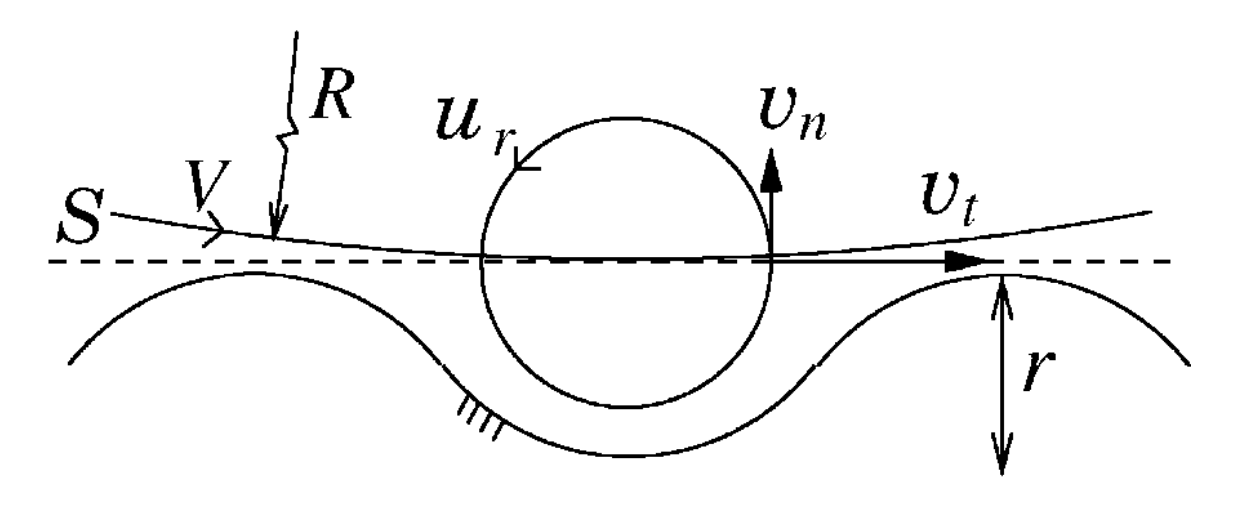
\includegraphics[width=0.5\textwidth]{./figures/eddies.png}
                % \caption{Schematic of eddy phenomenology \cite{gioiaprl2001}.}
                \label{fig:-figures-eddies-png}
            \end{figure}
        \end{column}
    \end{columns}
    \begin{itemize}
        \item Local wall shear stress model \cite{gioiaFriction2006}: $v_t \sim V$, $v_n\sim u_{r+a\eta}$
        \item Local water column shear stress model \cite{gioiaMVP2010}: $v_t\sim u(y+s) - u(y-s)\approx 2s u'(y) \sim 2y\cdot u'(y)$, $v_n \sim u_y$
    \end{itemize}
    \begin{figure}[!htb]
        \centering
        \begin{minipage}{.5\textwidth}
            \centering
            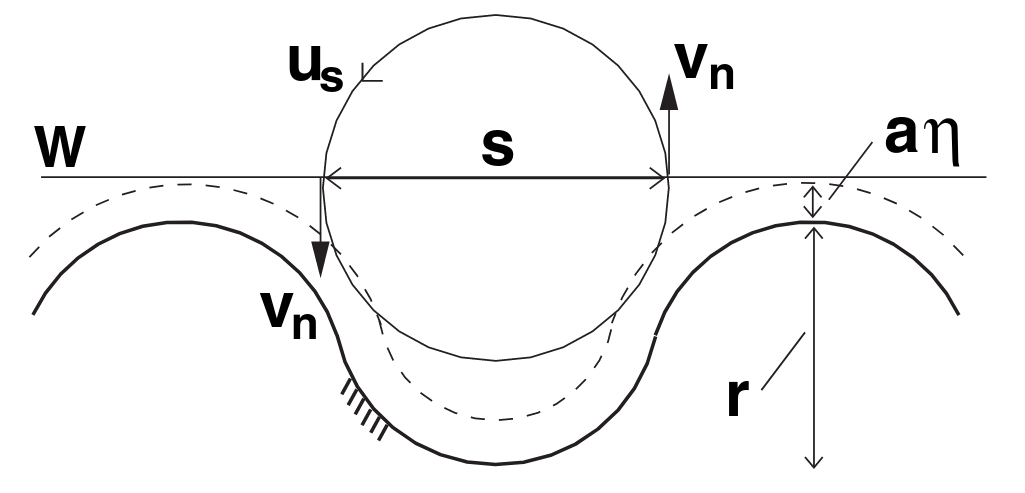
\includegraphics[width=0.6\textwidth]{./figures/wall-shear.png}
            \label{fig:wall-shear}
        \end{minipage}%
        \begin{minipage}{0.5\textwidth}
            \centering
            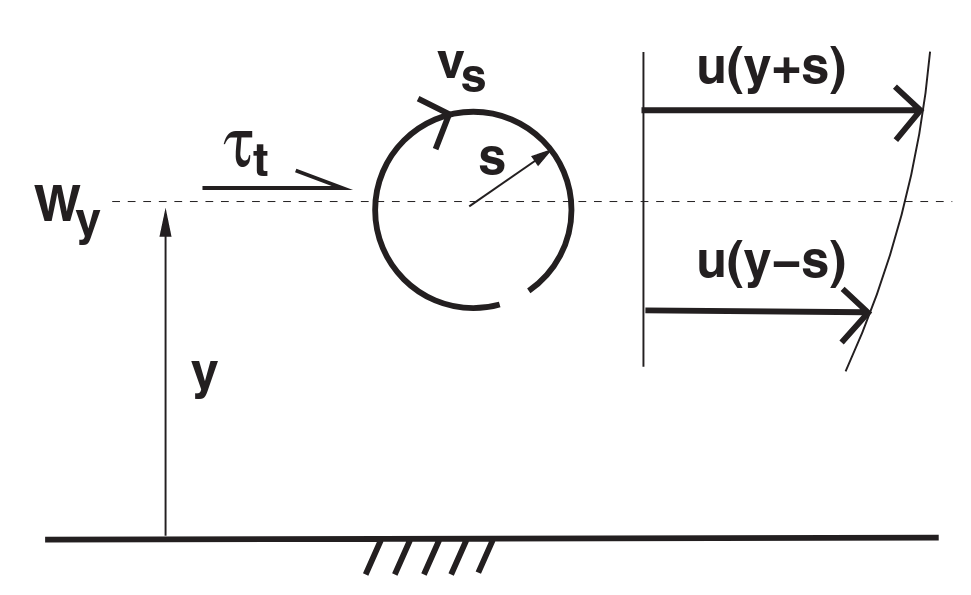
\includegraphics[width=0.6\textwidth]{./figures/column-shear.png}
            \label{fig:column-shear}
        \end{minipage}
    \end{figure}
\end{frame}

\begin{frame}{Unify the local shear stress model}
    \begin{figure}[htpb]
        \centering
        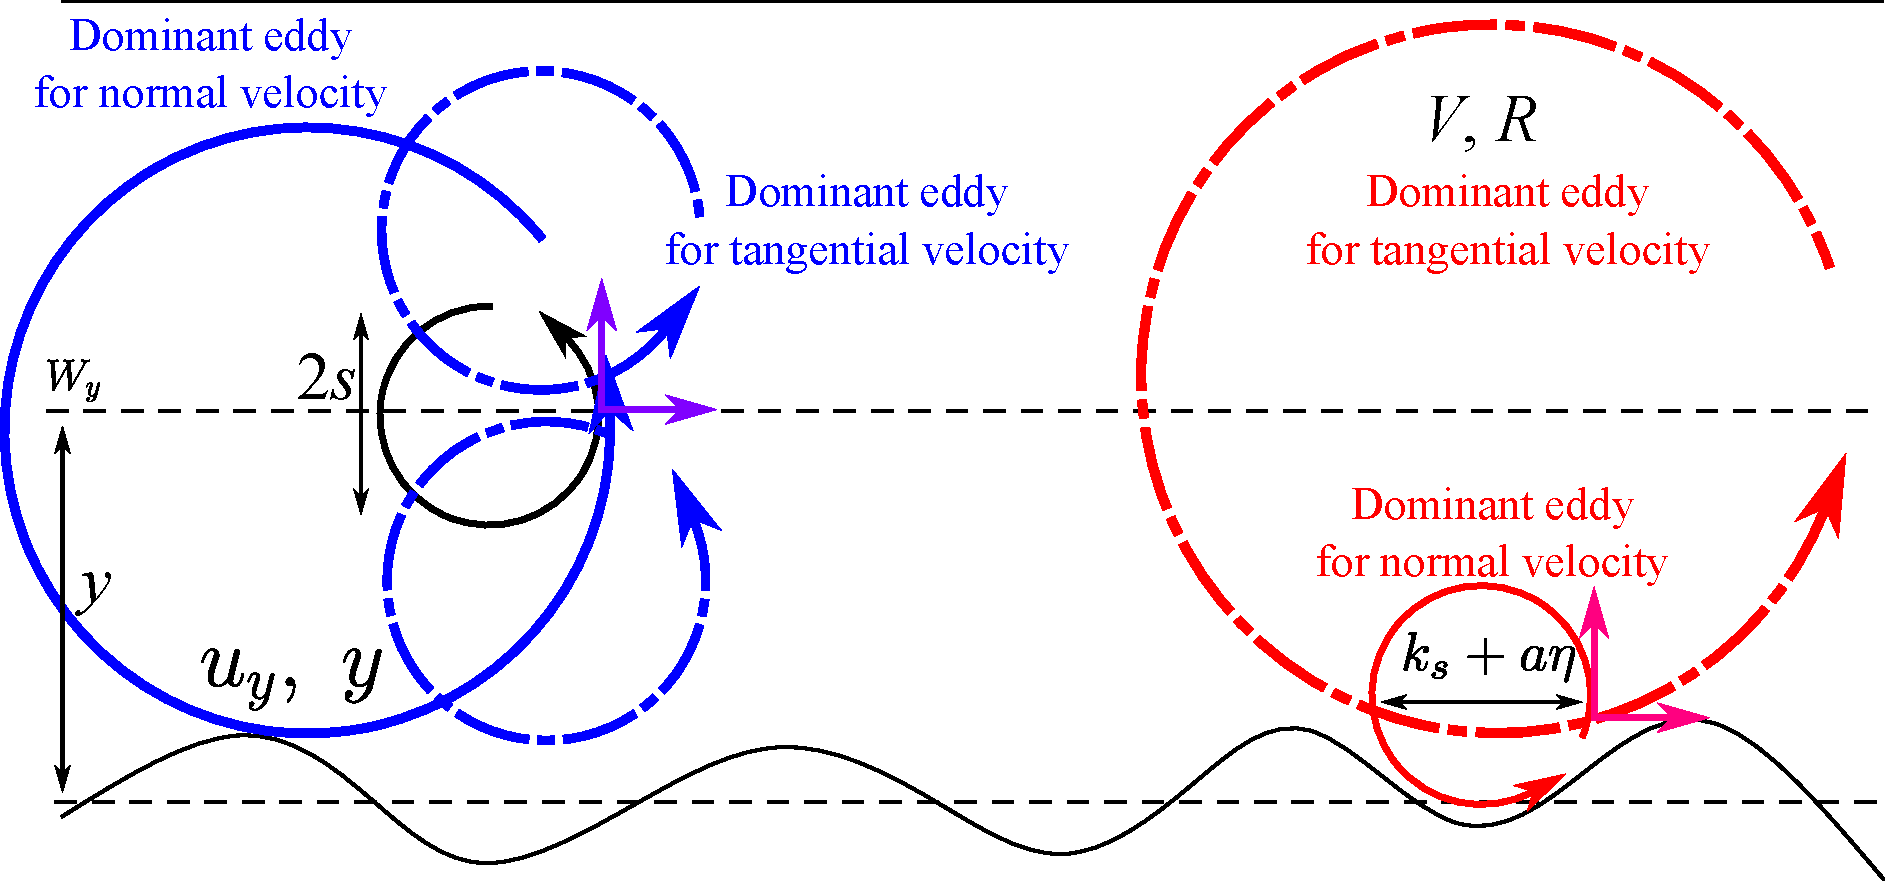
\includegraphics[width=0.8\textwidth]{./figures/unify-gioia-model.pdf}
        \caption{The unified picture of the Gioia model.}
        \label{fig:-figures-unify-gioia-model-pdf}
    \end{figure}
\end{frame}

\begin{frame}{Unify the local shear stress model}
    \begin{itemize}
        \item 搬运工$v_n$ :近床面位置,特征涡体由粗糙高度$k_s$ 和黏性底层$a\eta$ 共同控制 $s = k_s + a\eta$\ddag;外区部分的特征涡体完全由床面高度$s\sim y$ 控制\footnote{Townsend 附着涡模型存在类似的特征尺度正比于床面距离的一系列自相似涡体。或许可视作仅考虑外区涡体的特例,这导致附着涡模型仅适用于对数区\cite{aemmarusic2019}。}
        \item 货物$v_t$\his :提供$v_n$分量的涡体起到动量搬运工的作用,而其空间尺度决定\footnote{因为给定涡体空间尺度$s$,此距离覆盖的速度梯度是关于$s$ 的函数。}了其所能搬运的动量$v_t$ 
            \begin{itemize}
                \item 一旦涡体尺度$s$ 确定,$v_n$ 和$v_t$ 同时确定?那么大涡叠加小涡的模型不再必要,仅需引入搬运工涡体,与附着涡模型类似。
                \item 外区速度梯度引起的能够搬运的动量差 $$v_t \sim 2s u'(y) \sim 2y \cdot u'(y).$$
                \item 壁面附近的动量差\his \footnote{Strickler-type for transitional rough $\tau_0 \propto \left( k_s / R \right) ^{\frac{1}{3}} \rho V^2 $.}
                    $$\lim_{y \to 0} v_t \sim \left( k_s + a\eta \right) \lim_{y \to 0} u'(y) =  \frac{(k_s + a \eta)u_{\tau}^2}{\nu} \sim (k_s + a\eta) \frac{\left( k_s / R \right)^{\frac{1}{3}} V^2}{\nu}.$$
            \end{itemize}
    \end{itemize}
\end{frame}

\begin{frame}{Unify the local shear stress model}
    \begin{itemize}
        \item 一个涡体$\left( V, R \right) $ 代表一个动量扩散系统$\mathcal{D}_e \propto VR$ \cite{ocfjfm2024}\footnote{此时我们已经脱离流体可视化的视野,不再追求从流场中捕捉抽象的涡体。此处的视角与普朗特混合长度类似。}。越大的涡体扩散动能的能量越强。
            \begin{itemize}
                \item laminar flux is driven by molecular diffusion $\left( \propto \nu \right) $
                \item turbulent flow is driven by diffusion by the largest eddies and recirculation cells $\left( \propto VR \right) $
                \item $Re = \frac{VR}{\nu}$ 表示了湍流与层流驱动量的比值
            \end{itemize}
        \item 一个涡体$\left( V, R \right) $ 产生的动量通量$F$为\footnote{文章第二种情况的推导可能存在伪证的风险。} \cite{ocfjfm2024}
    \end{itemize}
    \begin{columns}
        \begin{column}{0.5\textwidth}
            \begin{align*}
                F \sim \rho \left[ (VR)^2 \right] '\sim -\rho \int_0^{R}  \mathcal{D}_e \frac{\partial u}{\partial y} dz
            .\end{align*}
        \end{column}
        \begin{column}{0.5\textwidth}
            \begin{figure}[htpb]
                \centering
                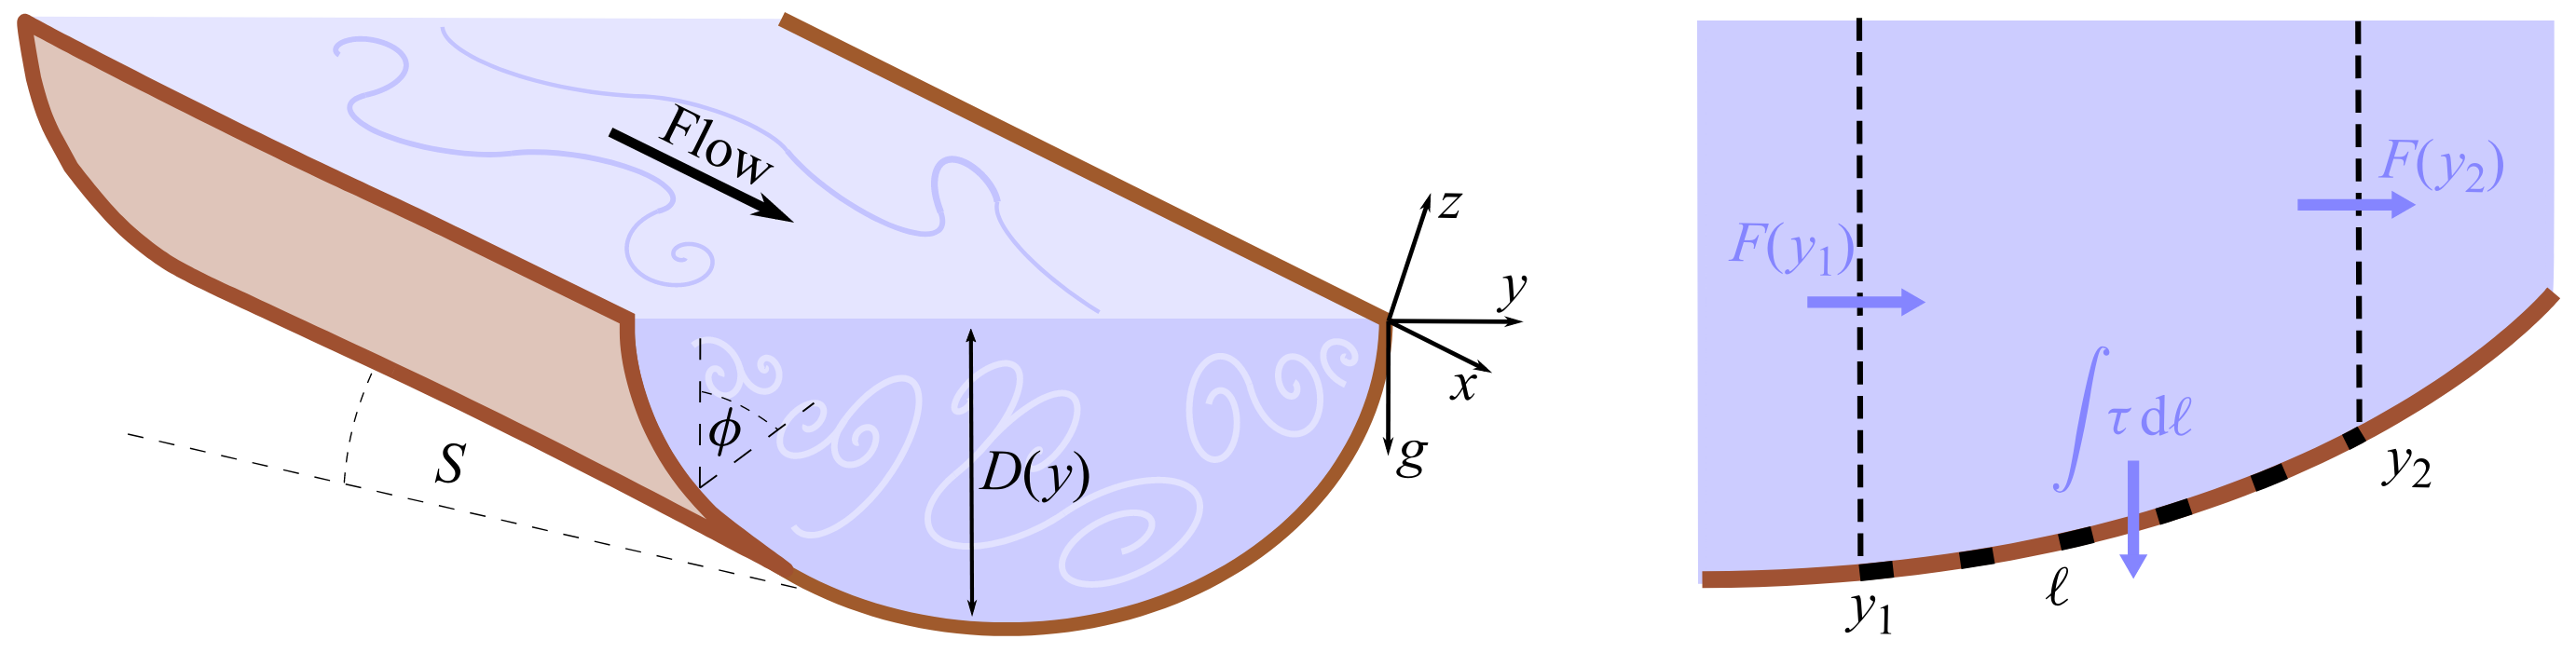
\includegraphics[width=0.85\textwidth]{./figures/momentum-flux.png}
                \caption{Momentum balance in a portion of the channel. \cite{ocfjfm2024}}
                \label{fig:-figures-momentum-flux-png}
            \end{figure}
        \end{column}
    \end{columns}
\end{frame}

\begin{frame}{The Gioia eddy model vs Attached eddy model}
    
\end{frame}

\begin{frame}{The Gioia eddy model vs Eddy viscosity model}
    
\end{frame}

\begin{frame}{HOWTO The Gioia eddy model in perspective of time average field}
    
\end{frame}

\begin{frame}{The Gioia eddy model vs LSM/VLSM}
    
\end{frame}

\begin{frame}{The vision}
    \begin{itemize}
        \item The local shear stress model $\implies$ sub-grid stress model
        \item New sub-grid stress model $\implies$ Mesh optimizer
    \end{itemize}
\end{frame}

\begin{frame}[allowframebreaks]
  \frametitle{参考文献}
  \printbibliography[heading=bibliography,title=参考文献]
  % \bibliographystyle{plain} % We choose the "plain" reference style
  % \bibliography{ref} % Entries are in the refs.bib file
\end{frame}

\end{document}
